\documentclass{standalone}
\usepackage{tikz}
\usetikzlibrary{patterns,decorations.pathmorphing}
\begin{document}
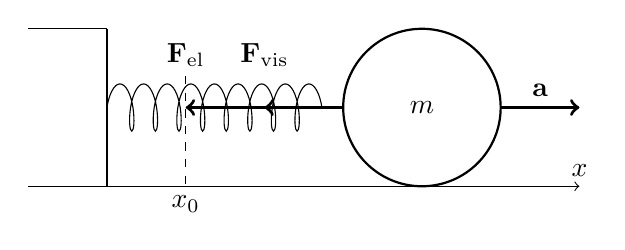
\begin{tikzpicture}[scale=2]
    \draw[->](-0.5,0)--(3,0)node[above]{$x$};
    \draw[-](0,0)--(0,1);
    \draw[-](0,1)--(-0.5,1);

    \draw[dashed](0.5,0.7)--(0.5,0)node[below]{$x_0$};

    \draw[->,very thick](1.5,0.5)--(0.5,0.5);
    \node[above]at(0.5,0.7){$\mathbf{F}_{\mathrm{el}}$};
    \draw[->,very thick](1.5,0.5)--(1,0.5);
    \node[above]at(1,0.7){$\mathbf{F}_\mathrm{vis}$};
    \node at(2,0.5){$m$};
    \draw[->,very thick](2.5,0.5)--(3,0.5)node[midway, above]{$\mathbf{a}$};

    \draw[decoration={aspect=0.3, segment length=3mm, amplitude=3mm,coil},decorate] (0,0.5) -- (1.5,0.5);
    \draw[thick](2,0.5)circle(0.5);
\end{tikzpicture}
\end{document}